%!TEX root = main.tex
%%%%%%%%%%%%%%%%%%%%%%%%%%%%%%%%%%%%%%%%%%%%%%%%%%%%%%%%%%%%%%%%%%%%%%%%%%%%%%%%

\section{Results}
\label{sec:results}


\subsection{optimal adaptation}

Idea: calculate the highest resolution that could have been achieved. compare it to measurement data. How much can still be gained?
opt was calculated according to the optimization problem in \cite{hossfeld2015identifying}. The calculations were done using the Gurobi Optimizer\footnote{http://www.gurobi.com/}.

\begin{figure}[t]
\centering
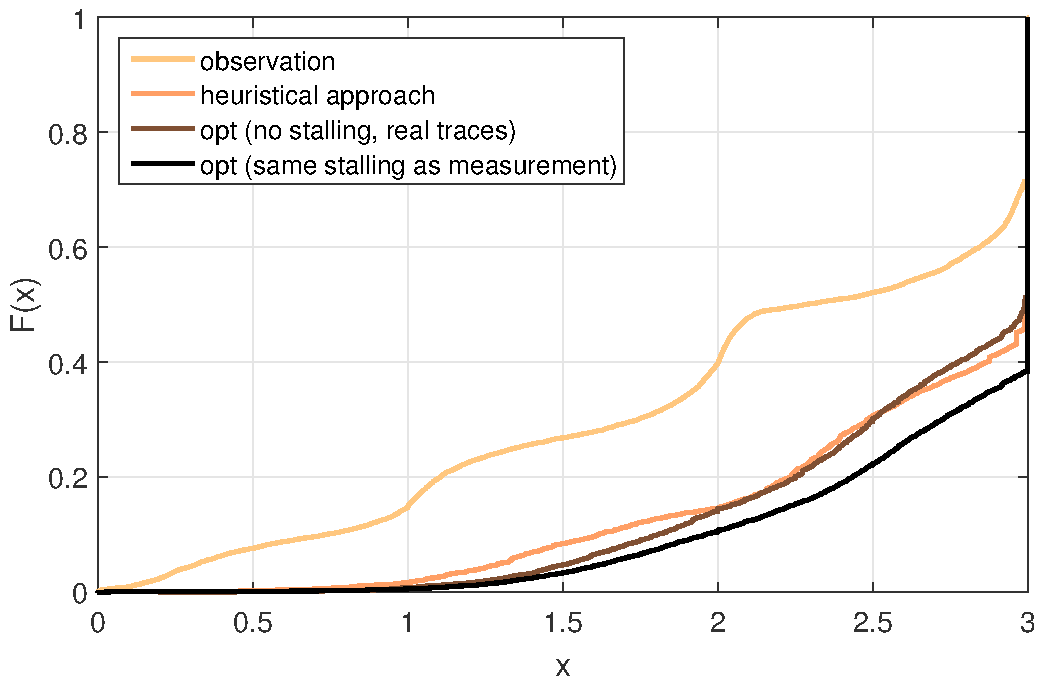
\includegraphics[width=0.5\textwidth]{figs/quality}%
\caption{CDF of the mean video quality in the measurement runs and highest achievable mean video quality according to the optimization problem in \cite{hossfeld2015identifying}. Remake figure!}
\label{fig:opt}%
\end{figure}

\begin{figure}[t]
\centering
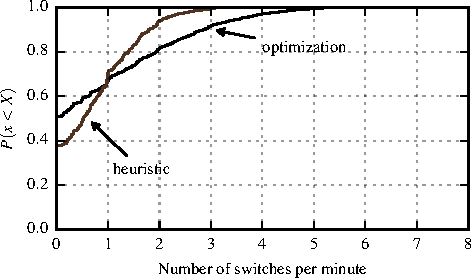
\includegraphics[width=0.5\textwidth]{figs/switches}%
\caption{CDF of the number of switches per minute. Remake figure!}
\label{fig:switches}%
\end{figure}

In figure \ref{fig:opt} we see the CDF of the mean video quality in the measurement runs and highest achievable mean video quality according to the optimization problem. In addition, we added an estimation of the avg. quality level that is possible based on downloaded data that was done in [BIEBnetworking2016]. While stalling events occured frequently during the original measurement, stalling events are not allowed to occur in the optimization problem. Therefore, we consider two sets of input for the opt. prob. for each measurement run: First, we only consider the available bandwidth during the video download. Second, we also respect the stalling events that occured. The sum of stalling was then added as initial delay during which the video was downloaded. In contrast to the YouTube measurement data where the video buffer does not contain more than 50s of video content at a time, in the calculations of the optimal adaptation we assumed that the video buffer is not limited.
